\documentclass[a4paper, 11pt]{article}
\usepackage[slovene]{babel}
\usepackage{comment} % enables the use of multi-line comments (\ifx \fi) 
\usepackage{lipsum} %This package just generates Lorem Ipsum filler text. 
\usepackage{fullpage} % changes the margin
\usepackage{graphicx}
\usepackage{url}
\usepackage[utf8]{inputenc}
\usepackage{amsfonts}
\usepackage[dvips]{psfrag}
\usepackage{fancyref}
\usepackage{graphicx}
\usepackage{epsfig}
\usepackage{amsmath}
\usepackage{amssymb}
\usepackage{tikz}
\usepackage{booktabs}


\graphicspath{{img/}}

\begin{filecontents*}{report.bib}
@MISC{WikipediaEN:IPI,
    author = {{Wikipedia, the free encyclopedia}},
    title = {Incubation preiod},
    year = {2017},
    note = {[Online; dostop 17 Avgust, 2017]},
    url = {https://upload.wikimedia.org/wikipedia/commons/0/04/Concept_of_incubation_period.svg}
}
\end{filecontents*}


\begin{document}
\noindent
\large\textbf{Poročilo o končnem projektu} \hfill \textbf{Filip Koprivec} \\
\normalsize Matematično modeliranje, 2016/2017 \hfill Vpisna številka: 27141059 \\


\section*{Navodila}
S pomočjo metode Monte Carlo analizirajte širjenje nalezljive bolezni na $2d$ mreži. Preverite, kako različni populacijski in bolezenski parametri (precepljenost, nalezljivost, smrtnost) vplivajo na širjenje bolezni in končno stanje.

\section*{Uvod}
Nalezljive bolezni so skozi zgodovino človeštva pomembno vplivale na celosten razvoj civilizacije in življenja posameznika. Skozi zgodovino je v kolektivnem spominu ostalo kar nekaj pomembnejših izbruhov nalezljivih bolezni (Črna smrt, ki je konec srednjega veka pomorila med 30 in 60\% evropskega prebivalstva, različne mrzlice, ki so ob prihodu Evropejcev ohromile prebilvastvo Amerik, do Španske gripe, ošpic in drugih.). Epidemije so s spreminjanjem populacijske dinamike pogosto močno spremenile tok zgodovine, bile pa so tudi pomemben razlog, ki je omejeval velikosti mest. Še celo v 19. stoletju sta bila tako London kot Pariz pogosto deležna izbruhov kolere, katerih vzrokov pa vse do razvoja teorije mikroorganizmov kot povzročiteljev bolezni ni bilo mogoče razložiti. V 20. stoletju pa je človeštvo z razvojem antibiotikov in cepiv mnoge izmed bolezni izkoreninili (črne koze, v Zahodnem svetu tudi očpice, rdečke in otroško paralizo).

Cepiva pa poleg odpornosti na bolezen prinašajo tudi stranske učinke, hkrati pa zaradi sestave ne smemo cepiti vseh prebivalcev določenega območja (alergija na učinkovino, alergija na beljakovine v cepivu itd.). Prav tako pa je določen del populacije vedno necepljen (novorojenčki do prejema cepiva, ljudje z osljabljenim imunskim sistemom, ljudje po presaditvi kostnega mozga, itd.). Klub temu pa lahko z dovolj veliko stopnjo precepljenosti vseeno zagotovimo tako imenovano čredno imunost, ko imuni posamezniki preprečujejo prenos bolezni do posameznikov, ki so dovzetni za okužbo. S pomočjo matematičnih modelov lahko tako preučujemo širjenje bolezni v populaciji glede na različne stopnje precepljenosti in pridemo do različnih zaključkov. Eden izmed zaključkov je lahko: pri kakšni stopnji precepljenosti je posamezna okužba (pri ustreznem ravnanju ob odkritju okužbe) omejena na manjše geografsko območje, kdaj pa kljub (sicer premajhnemu) deležu cepljenih pride do epidemije.

\section*{Analiza problema}
\subsection*{Različni modeli}
V projektni nalogi se osredotočimo na poenostavljen problem epidemije v populaciji. Zamislimo si zaprto populacijo (državo), v dovolj kratkem času, da normalni populacijski dejavniki ne pridejo do izraza (smrti, rojstva, emigracija). V veliki večini modeli populacijo razdelijo v več razdelkov. Eden izmed najbolj znanih (zveznih) modelov je tako imenovani SIR model, ki populacijo razdeli v tri dele: \emph{Susceptible} (osebki dovzetni za okužbo - zdravi), \emph{Infected} (okuženi osebki, ki lahko okužijo nove, ozdravijo, ali pa podležejo bolezni) in \emph{Removed} (osebki, ki so iz modela odstranjeni (se ne morejo okužiti), kot posledica smrti, lahko pa tudi kot posledica kakih drugih dejavnikov). Z nekaj malega znanja o biologiji lahko preprosto zapišemo sistem diferencialnih enačb za tak model:
\begin{align*}
	S' &= \Lambda(N) - \beta S I - \mu S \\
	I' &= \beta S I - \mu I -\alpha I  + \alpha I \\
	N' &= \Lambda(N) - (1-f)\alpha I - \mu N 
\end{align*}

Kjer je: $\Lambda(N)$ število rojstev, $\beta$ koeficient infektivnosti, $\mu$ splošna smrtnost, $\alpha$ smrtnost bolezni in $f$ delež osebkov, ki bolezen prebolijo z imunostjo. S pomočjo konstant lahko model kontroliramo. Pri večini modelov nas ne zanima celostna rešitev (ki je analitično navadno ne moremo dobiti), navadno je dovolj, če poznamo stacionarne točke, ter obnašanje v okolici. Vprašanje, ki se ga največkrat vprašamo je: Ali število okuženih hitro raste in so po dovolj dolgem časo okuženi vsi, ali se ustali pri nekem deležu populacije, ali pa bolezen odmre (po nekaj časa).

Naslednji razvoj modela je tako imenovani SIS model, ki bolje upošteva tudi dejstvo, da na nekeatere bolezni pridobimo imunost. Natančenjše analie modela tu ne bomo dodajali, je pa pomemben ker lahko določimo osnovno reprodukcijsko število ($R_0$), ki nam pove, kakšno je obnašanje števila okuženih po dovolj dolgem času.

\subsection*{Naključni model}
V svojem projektu sem si bolj podrobno ogledal simulacijski model. Predpostavimo fiksno število osebkov na 2d mreži, kjer vsakemu osebku priredimo svojo celico. Namesto na razdelkih populacije, simulacija deluje na nivoju posameznika, zato si lahko privoščimo nekoliko preurejen SEIR model, kjer posamezniku priredimo več značilnosti. Te značilnosti so podrobneje opisane tudi v kodi. Posamezniku priredimo več značilnosti, ki so pomembne za kužnost, prenosljivost in smrtnost bolezni:
\begin{enumerate}
\item \textbf{Startostna skupina}: Pomembna je zaradi učinkovitosti cepiv, smrtnosti pri različnih modelih, ter zaradi prenosljivosti. Ob bolj natančni simulaciji (za katero ni niti časa, niti procesorja, niti delovnega spomina), bi lahko s pomočjo starosti nadzorovali infektivnost posameznika zaradi različne razdalije potovanja (vožnja v sližbo), socialne skupine (otroci v šoli ali vrtcu so v stiku z velik drugimi otroci) in imajo v splošnem slabši imunski sistem, spolne aktivnosti, načina življenja, itd.
\begin{enumerate}
\item Otrok: do 14 let
\item Odrasel: od 15 do 64 let
\item Starejši: od 64 let naprej
\end{enumerate}

\item \textbf{Spol}: Spol je pomemben zaradi prenosljivosti različnih bolezni, smrtnosi, pri državah v razvoju tudi zaradi različnih socialnih krogov, ter ob simulacijah spolno prenosljivih bolezni.
\begin{enumerate}
\item Ženski
\item Moški
\end{enumerate}

\item \textbf{Status cepljenja}: S pomočjo bolj natančne razdelitve cepljenja lahko omogočimo simulacije, ki natančneje upoštevajo realno stanje, kjer določen delež cepiv ni učinkovit, ali pa so cepiva že stara, targetirajo drug sev bolezni (cepiva za gripo), ali pa so osebki sveže cepljeni.
\begin{enumerate}
\item Ni cepljen: posameznik ni cepljen, edina zaščita pred boleznijo je čredna imunost
\item Popolnoma cepljen: Posameznik je popolnoma cepljen, cepivo učinkuje, zanj ni verjetnosti da se naleze, saj je odporen na bolezen (dokler ne mutira)
\item Sveže cepljen: Sveže cepivo je navadno manj učinkovito, sa telo še ni povsem pripravljeno
\item Staro cepivo/drug sev: Cepivo je manj učinkovito, saj je staro, ali targetira drug sev bolezni
\item Nedelujoče cepivo: Pri večini cepiv določen delež posameznikov kljub cepljenu ni odporen (cepivo nu učinkovito), to stanje je enako kot Ni cepljen
\end{enumerate}

Poleg fizičnih lastnosti pa posamezniku glede na stanje obolelosti pripada še nekaj drugih značilnosti:

\item \textbf{Stanje infekcije}: V kakšnem stanju je pri posamezniku bolezen. Predvsem pomembna za ugotavljanje trenutnega stanja mreže.
\begin{enumerate}
\item Ni okužen: Posameznik (še) ni (bil) okužen
\item Trenutno okužen: Posameznik je trenutno okužen, simulacija poteka, dokler je vsaj še en posameznik okužen
\item Okužen v preteklosti: Posameznik je bil v preteklosti okužen, a je bolezen uspešno prebolel (lahko so sicer nastale komplikacije, a zaradi bolezni ni umrl). Model v osnovi predpostavi, da s tem posameznik pridobi imunost na nadaljne infekcije.
\item Mrtev: Posameznik je za posledicami bolezni umrl.
\end{enumerate}

\begin{figure}[h]
\caption{Grafični prikaz različnih stanj bolezni na časovni premici. Prevzeto iz \cite{wikiimg}.}
\label{img:incubation}
\centering
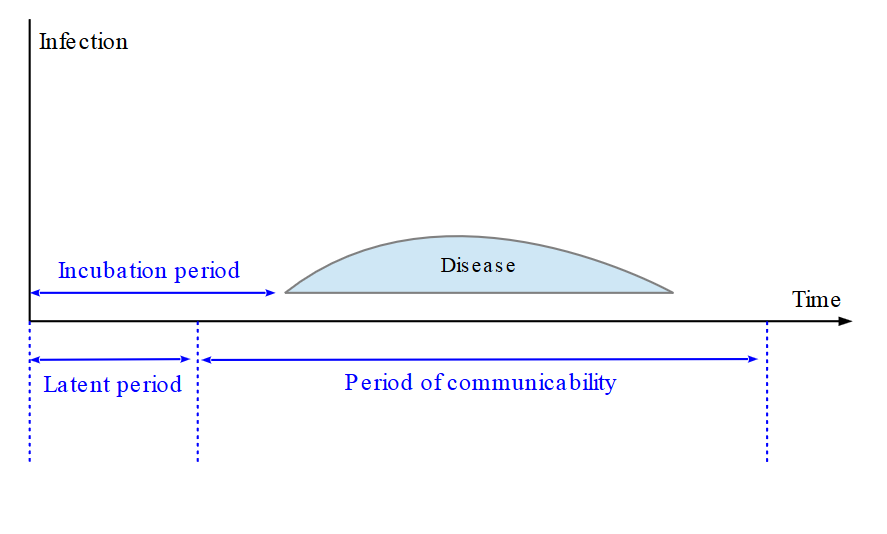
\includegraphics[width=1\textwidth]{incubation_concept.png}
\end{figure}

\item \textbf{Stanje bolezni}: V kakšnem simptomatskem stanju je pri posamezniku bolezen. Kljub temu da je posameznik okužen, je lahko bolezen nevidna (v inkubacijski dobi). Posameznik je sicer okužen, a ne kaže (vidnih) znakov okužbe. Tak posameznik je lahko vseeno kužen četudi ne kaže simptomov.
\begin{enumerate}
\item Inkubacijska doba: Posameznik je z boleznijo okužen, a ne kaže znakov (te se navadno pojavi nekaj dni(ošpice) po okužbi, pri nekaterih bolezni pa lahko to traja tudi več let ali desetletji(HIV, Kuru). 
\item Simptomatska doba: Posameznik je z boleznijo okužen in kaže simptome (fleki na koži, tresoče roke), kljub simpotomom posameznik ni nujno kužen.
\end{enumerate}

\item \textbf{Stanje nalezljivost}: Pove, ali je posameznik kužen ali ni. Odnos med simptomi in kužnostjo najlepše prikaže slika \ref{img:incubation}.
\begin{enumerate}
\item Ni kužen: Posameznik ni kužen
\item Kužen: Posameznik lahko okuži ljudi okoli sebe.
\end{enumerate}

\item \textbf{Trajanje bolezni}: Kako dolgo je posameznik okužen. S pomočjo tega parametra določamo kdaj posameznik postane kuže začne kazati simptome, ozdravi, itd.

\item \textbf{Dotaknjen}: Parameter je uporabljen za spremljanje poti epidemije. Vsakič ko posameznik pride v stik z okuženim (bi se potencialno lahko okužil) posameznik postane dotaknjen. S tem lahko spremljamo razširjenost epidemije in njeno napredovanje, ter možne varne točke.

\end{enumerate}

\section*{Optimum Solution}
\lipsum[4]
% to comment sections out, use the command \ifx and \fi. Use this technique when writing your pre lab. For example, to comment something out I would do:
%  \ifx
%	\begin{itemize}
%		\item item1
%		\item item2
%	\end{itemize}	
%  \fi

\section*{Construction/Implementation}
\lipsum[5]

\section*{Analysis \& Testing}
\lipsum[6]

\section*{Final Evaluation}
\lipsum[7]


\begin{thebibliography}{9}
\bibitem{math_models} BRAUER, Fred, in, CASTILLIO-CHÁVEZ, Carlos Castillo-Chávez \emph{Mathematical Models in Population Biology and Epidemiology}. New York: Springer-Verlag. ISBN: 978-1-4419-3182-5
\bibitem{Math_epidem}  BRAUER, Fred, et al. \emph{Mathematical Epidemilogy}. Heidelberg: Springer-Verlag. ISBN: 978-3-540-78910-9
\bibitem{articles} FENG, Zhilan, et al. \emph{Disease Evolution: Models, Concepts, and Data Analyses}. ISBN:0-8218-3753-2

\bibitem{wikiimg} Wikipedia, the free encyclopedia. Incubation period, 2017. URL https://upload.wikimedia.org/wikipedia/commons/0/04/Concept\textunderscore of\textunderscore incubation\textunderscore period.svg [Online; Datum dostopa 17. Avgust, 2017]
\end{thebibliography}


\hfill \textit{Filip Koprivec}


\end{document}
